\newpage
\section{Análisis de tecnologías}

Tal y como se puede ver en el capítulo anterior, hay una tendencia general a usar Typescript o Go para el desarrollo de el servidor de sincronización de multimedia y Flutter o PWA para el desarrollo de aplicaciones móviles debido a su popularidad y facilidad de uso.
Sin embargo, existen otras tecnologías que pueden ofrecer ventajas significativas en términos de rendimiento, seguridad y facilidad de desarrollo.


Se estudiarán las tecnologías disponibles para el desarrollo de la aplicación móvil, entre ellas React Native, Flutter, PWA y Lynx.js. Cada una de estas tecnologías tiene sus propias ventajas y desventajas, y la elección de la tecnología adecuada dependerá de los requisitos específicos del proyecto, como la necesidad de una experiencia de usuario nativa, el rendimiento en dispositivos móviles y la facilidad de desarrollo.

\subsection{Servidor}
El servidor de sincronización de multimedia es el componente central de la aplicación, encargado de gestionar la comunicación entre el cliente y el almacenamiento de fotos.
Disponemos de una amplia variedad a la hora de elegir un lenguaje/\gls{framework} para el desarrollo del servidor, cada uno con sus propias ventajas y desventajas.

Las principales soluciones serían:
\begin{itemize}
    \item \textbf{Node.js con TypeScript}: Muy popular, especialmente para aplicaciones web. Ofrece un ecosistema rico y una gran comunidad, siendo menos eficiente en términos de rendimiento y consumo de recursos con respecto a su competencia pero con una curva de aprendizaje más suave y una gran cantidad de bibliotecas disponibles.
    \item \textbf{Go}: Conocido por su eficiencia y facilidad de uso en aplicaciones concurrentes. Es una opción sólida para aplicaciones que requieren alto rendimiento y escalabilidad.
    \item \textbf{Rust}: Ofrece un alto rendimiento y seguridad en la gestión de memoria. Aunque tiene una curva de aprendizaje más pronunciada, es ideal para aplicaciones que requieren alta concurrencia y eficiencia.
    \item \textbf{C}: Lenguaje de bajo nivel con alto rendimiento, pero su complejidad y la gestión manual de memoria lo hacen menos adecuado para aplicaciones web modernas.
    \item \textbf{C++}: Similar a C, pero con características de programación orientada a objetos. Ofrece un alto rendimiento, pero su complejidad y la gestión manual de memoria lo hacen menos adecuado para aplicaciones web modernas.
    \item \textbf{Python}: Muy utilizado en el ámbito de la ciencia de datos y aprendizaje automático, pero menos eficiente en términos de rendimiento y escalabilidad para aplicaciones web, además de contar con un \gls{tipado-dinamico} que puede llevar a errores en tiempo de ejecución.
    \item \textbf{Java}: Aunque es robusto y escalable, su complejidad y consumo de recursos lo hacen menos atractivo para aplicaciones ligeras.
    \item \textbf{Ruby on Rails}: Muy popular para aplicaciones web, pero menos eficiente en términos de rendimiento y escalabilidad. No se ha trabajado mucho con esta tecnología, por lo que no se tiene una experiencia directa con ella.
\end{itemize}

A continuación se muestra una comparativa de rendimiento de los lenguajes anteriormente mencionados, en la cual se han medido el tiempo de CPU y el uso de memoria en tres algoritmos diferentes: Bubble Sort, Monte Carlo Pi y Monte Carlo Pi con un generador de números aleatorios simple (\texttt{SimpleRNG}).

\begin{figure}[H]
  \centering
  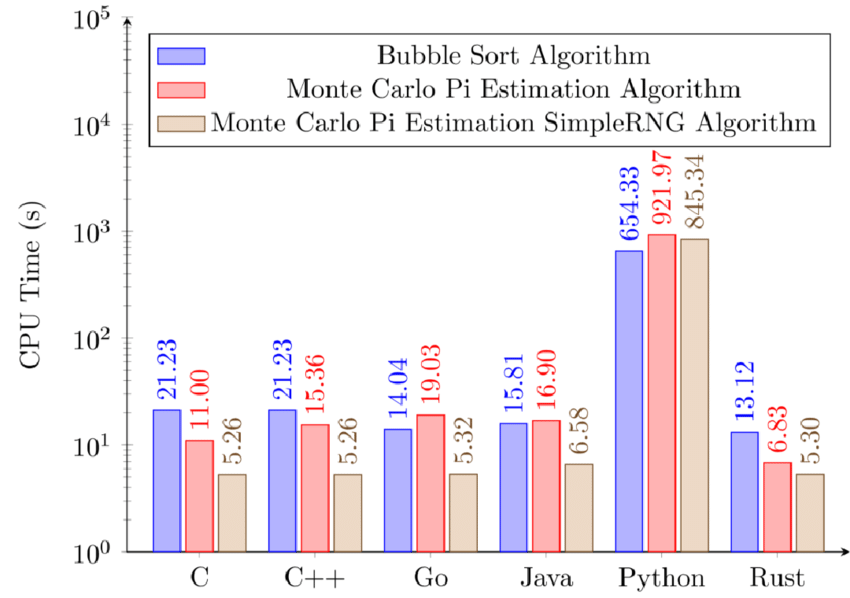
\includegraphics[width=0.8\textwidth]{assets/rust-cpu-comparison.png}
  \caption{Comparativa de uso de CPU entre Rust y otros lenguajes de programación (menos es mejor) \parencite{rust-for-safety-and-performance}}
  \label{fig:rust-cpu-comparison}
\end{figure}


\begin{figure}[H]
  \centering
  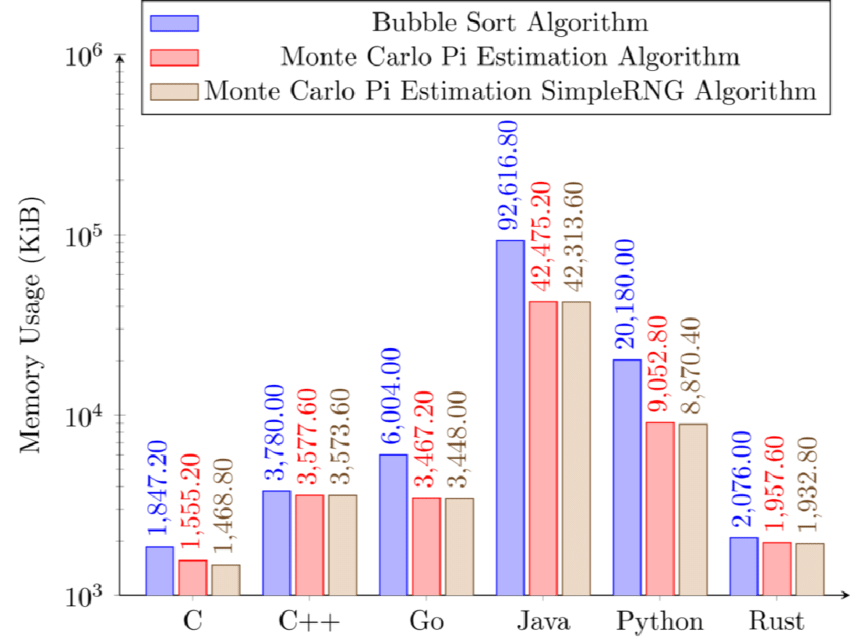
\includegraphics[width=0.8\textwidth]{assets/rust-memory-comparison.png}
  \caption{Comparativa de uso de memoria entre Rust y otros lenguajes de programación (menos es mejor) \parencite{rust-for-safety-and-performance}}
  \label{fig:rust-memory-comparison}
\end{figure}

Como se puede ver en las figuras \ref{fig:rust-cpu-comparison} y \ref{fig:rust-memory-comparison}, Rust tiene un rendimiento muy bueno en comparación con otros lenguajes de programación, tanto en uso de CPU como en uso de memoria.

A partir de las figuras, podemos definir dos fórmulas para calcular el porcentaje de mejora con respecto a los otros lenguajes de programación:
\begin{equation}
    \text{Mejora}_{\text{CPU}} (\%) = \left( \frac{T_{\text{\textit{lenguaje}}} - T_{\text{Rust}}}{T_{\text{\textit{lenguaje}}}} \right) \times 100
\end{equation}

\begin{equation}
    \text{Mejora}_{\text{Memoria}} (\%) = \left( \frac{M_{\text{\textit{lenguaje}}} - M_{\text{Rust}}}{M_{\text{\textit{lenguaje}}}} \right) \times 100
\end{equation}


Obteniendo las siguientes tablas de comparación:

\begin{table}[H]
\centering
\begin{tabular}{|c|c|c|c|}
\hline
\textbf{Lenguaje} & \textbf{Bubble Sort} & \textbf{Monte Carlo Pi} & \textbf{Monte Carlo Pi (SimpleRNG)} \\
\hline
C      & 38.2\%  & 37.9\%  & -0.8\% \\
C++    & 38.2\%  & 55.5\%  & -0.8\% \\
Go     & 6.5\%   & 64.1\%  & 0.4\%           \\
Java   & 17.0\%  & 59.6\%  & 19.4\%          \\
Python & 98.0\%  & 99.3\%  & 99.4\%          \\
\hline
\end{tabular}
\caption{Porcentaje de mejora de Rust con respecto a otros lenguajes de programación en términos de tiempo de CPU. (Mayor es mejor)}
\end{table}

\begin{table}[H]
\centering
\begin{tabular}{|c|c|c|c|}
\hline
\textbf{Lenguaje} & \textbf{Bubble Sort} & \textbf{Monte Carlo Pi} & \textbf{Monte Carlo Pi (SimpleRNG)} \\
\hline
C      & 89.8\%  & 20.4\%  & 25.6\%  \\
C++    & 45.1\%  & 45.3\%  & 45.9\%  \\
Go     & 65.4\%  & 43.5\%  & 44.0\%  \\
Java   & 97.8\%  & 95.4\%  & 95.4\%  \\
Python & 89.7\%  & 78.4\%  & 78.2\%  \\
\hline
\end{tabular}
\caption{Porcentaje de mejora de Rust con respecto a otros lenguajes de programación en términos de uso de memoria. (Mayor es mejor)}
\end{table}

Dado que para nuestro proyecto se busca la solución más eficiente (tanto en términos de velocidad como recursos) y segura, una vez vista la comparación entre las tecnologías candidatas, el análisis se puede reducir a una comparación entre Go y Rust, lenguajes que ofrecen un alto rendimiento y seguridad en la gestión de memoria.
Lenguajes como C, C++ han sido descartados puesto que, aunque ofrecen un alto rendimiento, su gestión de memoria es propensa a errores y fugas de memoria, lo que puede ser problemático en un desarrollo de código abierto y colaborativo.

Rust y Go son dos lenguajes de programación modernos que han ganado una popularidad considerable en los últimos años, especialmente en el desarrollo de sistemas y aplicaciones de alto rendimiento. Aunque ambos comparten objetivos como la eficiencia y la concurrencia, sus filosofías de diseño y enfoques para resolver problemas difieren significativamente.

\textbf{Rust} es un lenguaje de programación de sistemas enfocado en la seguridad de memoria y la concurrencia. Su principal objetivo es ofrecer el rendimiento de C/C++ sin los problemas comunes de gestión de memoria, como los punteros nulos o las \glspl{condicion-carrera}, gracias a su sistema de propiedad (\gls{rust-ownership}) y préstamos (\gls{rust-borrowing}).

\textbf{Go} (también conocido como Golang) es un lenguaje desarrollado por Google, diseñado para ser simple, eficiente y productivo, especialmente para la programación concurrente y de redes. Prioriza la simplicidad en su sintaxis y herramientas, facilitando una curva de aprendizaje suave.

\subsubsection{Gestión de Memoria}
\paragraph{Rust}
\subparagraph{}

Rust implementa un sistema de gestión de memoria único basado en los conceptos de \textit{ownership}, \textit{borrowing} y \textit{\glspl{rust-lifetimes}}. Este sistema garantiza la seguridad de memoria en tiempo de compilación sin necesidad de un \acrfull{gc}.

El sistema de gestión de memoria de Rust se basa en las siguientes reglas (\cite{rustbook2024} Capítulo 4):
\begin{itemize}
    \item Cada valor en Rust tiene un único propietario (owner).
    \item Cuando el propietario sale del ámbito, el valor se libera automáticamente.
    \item Los valores pueden ser prestados (borrowed) de forma mutable o inmutable, pero no ambos al mismo tiempo.
    \item Solamente puede haber un préstamo mutable o múltiples préstamos inmutables a un valor al mismo tiempo. Un préstamo mutable no puede existir a la vez que un préstamo inmutable, dado que podría llevar a condiciones de carrera.
    \item Los préstamos tienen una duración (lifetime) que garantiza que los datos referenciados sigan siendo válidos durante su uso. El tiempo de vida de los préstamos se determina en tiempo de compilación, lo que evita errores comunes de punteros nulos o dangling pointers.
\end{itemize}

Gracias a ello, tenemos control preciso sobre la memoria, ausencia de pausas por GC, prevención de fugas de memoria y carreras de datos de forma estática. El compilador será muy estricto, lo que hará que prevengamos errores en tiempo de ejecución.

Todo este paradigma de programación es totalmente distinto a lo que estamos acostumbrados en otros lenguajes de programación como puede ser Java o c++/c, lo que puede llevar a una curva de aprendizaje más pronunciada, pero a largo plazo nos va a permitir desarrollar aplicaciones más seguras y eficientes.

\paragraph{Go}
\subparagraph{}

Go utiliza un recolector de basura para la gestión automática de la memoria. Este GC está optimizado para baja latencia, aunque introduce ciertas pausas (\cite{go-documentation}, The Go Memory Model).

Go está diseñado para ser un lenguaje de programación lo más eficiente posible para concurrencia, por lo que su modelo de memoria también está optimizado para facilitar la programación concurrente. Utiliza un modelo de memoria basado en \glspl{csp} (Communicating Sequential Processes \cite{communicating-sequential-processes}), donde las goroutines (hilos ligeros) se comunican a través de canales, evitando la necesidad de compartir memoria directamente.
\begin{itemize}
    \item \textbf{Ventajas:} Simplifica la gestión de memoria para el desarrollador, haciendo más sencillo el desarrollo de aplicaciones concurrentes. El lenguaje es más fácil de aprender y usar, especialmente para principiantes.
    \item \textbf{Desventajas:} Introduce una sobrecarga (overhead) y posibles pausas no determinísticas debido al GC, lo que puede ser un inconveniente en aplicaciones de tiempo real estricto.
\end{itemize}

\subsubsection{Rendimiento}
\paragraph{Rust}
\subparagraph{}
Rust está diseñado para ofrecer un rendimiento comparable al de C y C++. Sus abstracciones de ``coste cero'' aseguran que las características de alto nivel no impongan una penalización en tiempo de ejecución. La ausencia de GC también contribuye a un rendimiento predecible.

Rust ofrece varias abstracciones de coste cero como \texttt{iterators}, \texttt{closures} y \texttt{async/await} que permiten escribir código limpio y expresivo sin sacrificar el rendimiento. Además, su sistema de tipos y el modelo de propiedad permiten al compilador realizar optimizaciones agresivas que en otro lenguaje son imposibles.

En el rendimiento podemos distinguir entre dos aspectos:
\begin{itemize}
    \item \textbf{Compilación:} Los tiempos de compilación pueden ser más largos debido a las exhaustivas verificaciones que realiza el compilador.
    \item \textbf{Ejecución:} Muy alta velocidad de ejecución y uso eficiente de los recursos gracias a su modelo de propiedad.
\end{itemize}

\paragraph{Go}
\subparagraph{}

Go ofrece un buen rendimiento, aunque generalmente no alcanza el nivel de Rust o C++ en tareas que requieren máxima optimización a bajo nivel. Su compilador es notablemente rápido en comparación con el de Rust, dado que está enfocado a solucionar errores en ejecución y no en compilación.

Go utiliza un modelo de concurrencia basado en \glspl{goroutine} y canales (\cite{go-documentation}, The Go Memory Model), lo que permite un alto grado de paralelismo sin complicaciones adicionales. Esto lo hace ideal para aplicaciones que requieren manejar múltiples tareas simultáneamente, como servidores web o servicios de red.

\begin{itemize}
    \item \textbf{Compilación:} Tiempos de compilación muy rápidos, lo que agiliza el ciclo de desarrollo.
    \item \textbf{Ejecución:} Buen rendimiento para la mayoría de las aplicaciones, especialmente en \acrshort{i-o} y concurrencia. El GC puede impactar el rendimiento en ciertos escenarios.
\end{itemize}

\subsubsection{Concurrencia}
\paragraph{Rust}
\subparagraph{}

Rust aborda la concurrencia con un enfoque en la seguridad (``\gls{fearless-concurrency}'', \cite{rustbook2024}, Capítulo 16), el cual permite realizar operaciones concurrentes sin preocuparse por problemas usuales de la concurrencia como pueden ser las condiciones de carrera.
Su sistema de tipos y el modelo de propiedad previenen las carreras de datos en tiempo de compilación.
Utiliza primitivas como \texttt{async/await} para la programación asíncrona, además de hilos de sistema operativo, consiguiendo paralelismo para la programación asíncrona.

Rust permite la creación de hilos seguros y eficientes, y su modelo de propiedad garantiza que no haya condiciones de carrera. El compilador verifica en tiempo de compilación que no se acceda a datos compartidos de forma insegura gracias a su modelo de propiedad de variables, lo que reduce significativamente los errores comunes en la programación concurrente.
\begin{itemize}
    \item \textbf{Ventajas:} Concurrencia segura sin condiciones de carrera garantizada por el compilador. Buen soporte para paralelismo.
    \item \textbf{Desventajas:} La programación concurrente puede ser más verbosa o compleja de configurar inicialmente en comparación con Go.
\end{itemize}

\paragraph{Go}
\subparagraph{}

La concurrencia es una de las características estrella de Go. Se basa en \textit{goroutines} y \textit{canales} (channels) para la comunicación entre goroutines, siguiendo el paradigma de \acrfull{csp}.
Éste se basa en la idea de que las goroutines se comunican entre sí a través de canales sin acceder a las mismas posiciones de memoria (cada goroutine tiene su propia copia de el mensaje) y reduce el riesgo de condiciones de carrera.
Si queremos tener una comunicación bidireccional, tendríamos que utilizar un enfoque más tradicional mediante \glspl{mutex} o \glspl{semaforo} junto con \glspl{lock}, lo cual puede ser más complejo y propenso a errores.
\begin{itemize}
    \item \textbf{Ventajas:} Modelo de concurrencia muy simple y potente. Facilidad para escribir software concurrente y paralelo.
    \item \textbf{Desventajas:} Aunque las goroutines son ligeras, una mala gestión puede llevar a problemas de rendimiento o fugas de goroutines. Las condiciones de carrera son posibles y deben ser manejadas por el desarrollador.
\end{itemize}

\subsubsection{Sintaxis y Curva de Aprendizaje}
\paragraph{Rust}
\subparagraph{}
La sintaxis de Rust es moderna y expresiva, pero su sistema de tipos y el modelo de gestión de memoria (ownership y borrowing) introducen una curva de aprendizaje considerablemente más pronunciada que la de Go.
Ya se ha trabajado anteriormente con Rust, lo cual facilita el aprendizaje de este lenguaje.
Además, la documentación oficial de Rust es muy completa y está bien estructurada, contando con el libro oficial de rust \parencite{rustbook2024}, que ayuda a los nuevos usuarios a familiarizarse con el lenguaje.
\begin{itemize}
    \item \textbf{Ventajas:} Sintaxis potente que permite un control muy granular.
    \item \textbf{Desventajas:} Dificultad inicial alta para dominar los conceptos clave.
\end{itemize}

\paragraph{Go}
\subparagraph{}

Go fue diseñado con la simplicidad como uno de sus principios fundamentales. Su sintaxis es minimalista y fácil de aprender, especialmente para programadores con experiencia en lenguajes tipo C.
\begin{itemize}
    \item \textbf{Ventajas:} Curva de aprendizaje suave, alta legibilidad y productividad rápida.
    \item \textbf{Desventajas:} La simplicidad puede llevar a cierta verbosidad en algunos casos (por ejemplo, el manejo de errores antes de la versión 1.13 con \texttt{wrap error}). Algunos patrones comunes de otros lenguajes no tienen un equivalente directo.
\end{itemize}

\subsubsection{Sistema de Tipos y Abstracciones}
\paragraph{Rust}
\subparagraph{}

Rust posee un sistema de tipos estático, fuerte y muy rico, inspirado en lenguajes como \gls{haskell}. Incluye \textit{\gls{rust-traits}}, genéricos avanzados, \acrlong{adt} \gls{adt-gls} como \texttt{enum} y \texttt{struct} que, gracias a el \gls{pattern-matching} y el coste cero, nos permite un desarrollo muy expresivo y seguro.
\begin{itemize}
    \item \textbf{Ventajas:} Gran expresividad, seguridad de tipos, permite abstracciones potentes y seguras.
    \item \textbf{Desventajas:} Puede resultar complejo para quienes vienen de lenguajes con sistemas de tipos más simples.
\end{itemize}

\paragraph{Go}
\subparagraph{}

Go tiene un sistema de tipos estático y simple. Utiliza interfaces para la polimorfismo de forma implícita (tipado estructural). Los genéricos fueron añadidos en la versión 1.18, lo que ha expandido sus capacidades de abstracción.
\begin{itemize}
    \item \textbf{Ventajas:} Simplicidad en el sistema de tipos, interfaces fáciles de usar. La adición de genéricos ha mejorado la reutilización de código.
    \item \textbf{Desventajas:} Menos expresivo que el sistema de tipos de Rust. Antes de los genéricos, la falta de ellos era una limitación importante.
\end{itemize}

\subsubsection{Ecosistema y Herramientas}
\paragraph{Rust}
\subparagraph{}

Rust cuenta con \textbf{Cargo}, una herramienta de gestión de dependencias y construcción de proyectos muy elogiada. El repositorio oficial de paquetes es \textbf{crates.io}, que alberga una cantidad creciente de bibliotecas.

Cargo además ofrece herramientas integradas para pruebas, documentación y gestión de versiones.
\begin{itemize}
    \item \textbf{Ventajas:} Herramientas robustas y unificadas. Comunidad activa y creciente.
    \item \textbf{Desventajas:} Aunque el ecosistema está creciendo rápidamente, puede no ser tan maduro como el de Go en ciertas áreas específicas (ej. algunas bibliotecas para servicios web muy específicos).
\end{itemize}

\paragraph{Go}
\subparagraph{}

Go posee una excelente librería estándar que cubre muchas necesidades comunes, especialmente en networking y servicios web. Sus herramientas de desarrollo (formateo, testing, profiling) están integradas en la distribución del lenguaje. Utiliza módulos de Go para la gestión de dependencias.
\begin{itemize}
    \item \textbf{Ventajas:} Librería estándar muy completa. Herramientas simples y efectivas. Compilación cruzada sencilla.
    \item \textbf{Desventajas:} Menor cantidad de bibliotecas de terceros para ciertos dominios muy especializados en comparación con lenguajes más antiguos, aunque el ecosistema es maduro para sus casos de uso principales.
\end{itemize}

\subsubsection{Manejo de Errores}
\paragraph{Rust}
\subparagraph{}
Rust no utiliza excepciones. El manejo de errores se realiza principalmente a través de los tipos \texttt{Result<T, E>} y \texttt{Option<T>} y el pattern matching exhaustivo, que obligan al programador a considerar los casos de éxito y error explícitamente, sin posibilidad de compilar si no se manejan los errores correctamente.
\begin{itemize}
    \item \textbf{Ventajas:} Manejo de errores robusto y explícito, que previene errores no gestionados.
    \item \textbf{Desventajas:} Puede resultar verboso en comparación con las excepciones, aunque el operador \texttt{?}\footnote{El operador ? devuelve el error si ocurre sin necesidad de introducir un \textit{match}} ayuda a mitigar esto.
\end{itemize}

\paragraph{Go}
\subparagraph{}
Go maneja los errores retornándolos como el último valor de una función. Por convención, un error es un valor que satisface la interfaz \texttt{error}. Esto requiere comprobaciones explícitas \texttt{if err != nil}.
El manejo de errores en este caso no es exhaustivo.
\begin{itemize}
    \item \textbf{Ventajas:} Simple y explícito.
    \item \textbf{Desventajas:} Puede llevar a código repetitivo y verboso con múltiples comprobaciones de error.
\end{itemize}

\subsubsection{Casos de Uso Principales}
\paragraph{Rust}

\begin{itemize}
    \item Programación de sistemas (sistemas operativos, navegadores web).
    \item Motores de videojuegos.
    \item \acrfull{cli}.
    \item Desarrollo en \gls{webassembly} (WASM).
    \item Sistemas embebidos.
    \item Aplicaciones que requieren alto rendimiento y seguridad de memoria.
\end{itemize}

\paragraph{Go}

\begin{itemize}
    \item Servicios de backend y microservicios.
    \item Herramientas de red y servidores.
    \item Herramientas de \gls{devops} y CLI.
    \item Bases de datos distribuidas.
    \item Aplicaciones concurrentes.
\end{itemize}

\subsubsection{Resumen de Ventajas y Desventajas}

\paragraph{Rust}
\subparagraph{Ventajas:}
\begin{itemize}
    \item Seguridad de memoria sin recolector de basura.
    \item Alto rendimiento, comparable a C/C++.
    \item Concurrencia segura ("fearless concurrency").
    \item Sistema de tipos rico y expresivo.
    \item Excelente gestor de paquetes y herramientas (Cargo).
    \item Creciente popularidad en dominios críticos.
\end{itemize}
\textbf{Desventajas:}
\begin{itemize}
    \item Curva de aprendizaje pronunciada.
    \item Tiempos de compilación más lentos.
    \item Mayor verbosidad en algunos aspectos debido a la gestión de memoria y errores.
\end{itemize}

\paragraph{Go}
\subparagraph{Ventajas:}

\begin{itemize}
    \item Simplicidad y facilidad de aprendizaje.
    \item Modelo de concurrencia simple y potente (goroutines, channels).
    \item Tiempos de compilación muy rápidos.
    \item Librería estándar robusta.
    \item Buena productividad para el desarrollo de servicios de red.
    \item Respaldo de Google y una comunidad madura.
\end{itemize}
\textbf{Desventajas:}
\begin{itemize}
    \item Rendimiento generalmente inferior a Rust en cómputo intensivo.
    \item El recolector de basura puede introducir latencias.
    \item El sistema de tipos es menos expresivo que el de Rust (aunque mejorado con genéricos).
    \item El manejo de errores puede ser verboso.
\end{itemize}


\subsection{Aplicación Móvil}

Para el desarrollo de aplicaciones móviles en el contexto de bibliotecas de archivos multimedia, existen varias tecnologías que ofrecen diferentes enfoques y características. A continuación se presenta un análisis detallado de las principales opciones disponibles.

\paragraph{React Native}

React Native, desarrollado por Meta (Facebook), permite crear aplicaciones móviles nativas utilizando JavaScript y React. Es ampliamente adoptado en la industria y cuenta con un ecosistema maduro.

\textbf{Arquitectura y Funcionamiento:}
\begin{itemize}
    \item Utiliza un \gls{bridge} para comunicar JavaScript con componentes nativos
    \item Renderiza componentes nativos reales, no WebViews
    \item Permite integración de código nativo cuando es necesario
    \item Soporte para hot reload durante el desarrollo
\end{itemize}

\textbf{Ventajas:}
\begin{itemize}
    \item \textbf{Ecosistema maduro}: Gran cantidad de bibliotecas y componentes disponibles
    \item \textbf{Comunidad activa}: Amplio soporte de la comunidad y documentación extensa
    \item \textbf{Desarrollo rápido}: Reutilización de código entre iOS y Android (70-80\%)
    \item \textbf{Performance nativa}: Acceso directo a APIs nativas del dispositivo
    \item \textbf{Flexibilidad}: Posibilidad de escribir módulos nativos cuando sea necesario
\end{itemize}

\textbf{Desventajas:}
\begin{itemize}
    \item \textbf{Bridge overhead}: La comunicación JavaScript-nativo puede introducir latencias
    \item \textbf{Tamaño de aplicación}: Las aplicaciones tienden a ser más grandes debido a las dependencias
    \item \textbf{Fragmentación}: Diferentes versiones pueden tener incompatibilidades
    \item \textbf{Limitaciones de UI}: Algunos componentes complejos requieren implementación nativa
\end{itemize}

\paragraph{Flutter}

Flutter, desarrollado por Google, utiliza el lenguaje Dart y un enfoque único de renderizado que dibuja todos los componentes desde cero utilizando \gls{skia}.

\textbf{Arquitectura y Funcionamiento:}
\begin{itemize}
    \item Engine compilado en C++ que renderiza directamente con Skia
    \item Framework en Dart que gestiona widgets y estado
    \item Compilación \gls{ahead-of-time} (AOT) para producción
    \item Hot reload y hot restart para desarrollo
\end{itemize}

\textbf{Ventajas:}
\begin{itemize}
    \item \textbf{Rendimiento consistente}: 60\acrshort{fps} garantizados en la mayoría de dispositivos
    \item \textbf{UI personalizable}: Control total sobre cada píxel de la interfaz
    \item \textbf{Consistencia multiplataforma}: Misma apariencia en iOS y Android
    \item \textbf{Desarrollo productivo}: \Gls{hot-reload} extremadamente rápido
    \item \textbf{Compilación nativa}: Sin bridge, comunicación directa con APIs nativas
\end{itemize}

\textbf{Desventajas:}
\begin{itemize}
    \item \textbf{Curva de aprendizaje}: Dart es menos conocido que JavaScript
    \item \textbf{Tamaño de aplicación}: El engine de Flutter añade peso significativo (4-8MB base)
    \item \textbf{Ecosistema más joven}: Menos bibliotecas de terceros comparado con React Native
    \item \textbf{Plataformas específicas}: Algunas funcionalidades requieren plugins específicos
    \item \textbf{Limitaciones de integración}: Puede ser complicado integrar con código nativo existente
    \item \textbf{Renderizado sobre motor gráfico}: Dado que no renderiza de manera nativa, puede ser menos eficiente en dispositivos de gama baja
\end{itemize}

\paragraph{Progressive Web Apps (PWA)}

Las PWA representan una evolución de las aplicaciones web tradicionales, ofreciendo características similares a las aplicaciones nativas mediante tecnologías web estándar.

\textbf{Arquitectura y Funcionamiento:}
\begin{itemize}
    \item \Glspl{service-worker} para funcionalidad offline y caché
    \item Web App Manifest para instalación y apariencia nativa
    \item Responsive design para adaptación a diferentes dispositivos
    \item APIs web modernas para acceso a funcionalidades del dispositivo
\end{itemize}

\textbf{Ventajas:}
\begin{itemize}
    \item \textbf{Desarrollo unificado}: Una sola base de código para web y móvil
    \item \textbf{Distribución sencilla}: No requiere app stores, actualización automática
    \item \textbf{Peso reducido}: Generalmente más ligeras que aplicaciones nativas
    \item \textbf{Accesibilidad}: Funcionan en cualquier dispositivo con navegador moderno
    \item \textbf{SEO}: Indexables por motores de búsqueda
\end{itemize}

\textbf{Desventajas:}
\begin{itemize}
    \item \textbf{Limitaciones de API}: Acceso restringido a funcionalidades nativas
    \item \textbf{Rendimiento}: Inferior a aplicaciones nativas para tareas intensivas
    \item \textbf{Experiencia de usuario}: Puede sentirse menos "nativa"
    \item \textbf{Soporte variable}: Diferencias de implementación entre navegadores
    \item \textbf{Distribución}: Menor visibilidad sin presencia en app stores
\end{itemize}

\paragraph{Lynx.js}

Lynx.js representa una tecnología emergente que promete combinar el desarrollo web con el rendimiento nativo, aunque su adopción y madurez son significativamente menores que las alternativas establecidas.

\textbf{Arquitectura y Funcionamiento:}
\begin{itemize}
    \item Runtime nativo que ejecuta JavaScript sin WebView
    \item Compilación just-in-time optimizada para móviles
    \item Bridge optimizado para comunicación JavaScript-nativo
    \item Soporte para APIs nativas modernas
    \item Uso de doble thread para mejorar el rendimiento y experiencia de usuario
\end{itemize}

\textbf{Ventajas:}
\begin{itemize}
    \item \textbf{Rendimiento optimizado}: Promete mejor rendimiento que React Native gracias a su ejecución con doble thread
    \item \textbf{Tamaño reducido}: Runtime más ligero que Flutter
    \item \textbf{Desarrollo familiar}: Utiliza JavaScript/TypeScript estándar
    \item \textbf{APIs modernas}: Soporte nativo para funcionalidades actuales
    \item \textbf{Interoperabilidad}: Posibilidad de integrar código nativo fácilmente, de manera similar a React Native
    \item \textbf{Actualizaciones}: Desarrollado y utilizado por el equipo de TikTok, lo que promete actualizaciones y mejoras constantes
\end{itemize}

\textbf{Desventajas:}
\begin{itemize}
    \item \textbf{Tecnología inmadura}: Ecosistema limitado y documentación escasa
    \item \textbf{Comunidad pequeña}: Pocos recursos y ejemplos disponibles
    \item \textbf{Estabilidad}: Versiones alpha/beta con cambios frecuentes
    \item \textbf{Compatibilidad}: Posibles problemas con bibliotecas existentes
\end{itemize}

\subsection{Comparación de Tecnologías Móviles}

\begin{table}[H]
\centering
\begin{tabular}{|l|c|c|c|c|}
\hline
\textbf{Criterio} & \textbf{React Native} & \textbf{Flutter} & \textbf{PWA} & \textbf{Lynx.js} \\
\hline
Rendimiento & 7/10 & 9/10 & 5/10 & 8/10* \\
Ecosistema & 9/10 & 8/10 & 8/10 & 3/10 \\
Curva Aprendizaje & 6/10 & 7/10 & 9/10 & 7/10 \\
Tamaño App & 6/10 & 5/10 & 9/10 & 8/10* \\
Acceso Nativo & 9/10 & 9/10 & 4/10 & 8/10* \\
Desarrollo Rápido & 8/10 & 9/10 & 9/10 & 6/10 \\
Estabilidad & 9/10 & 8/10 & 8/10 & 4/10 \\
Comunidad & 9/10 & 8/10 & 7/10 & 2/10 \\
\hline
\multicolumn{5}{|l|}{*Datos basados en especificaciones, experiencia limitada} \\
\hline
\end{tabular}
\caption{Comparación de tecnologías para desarrollo móvil}
\label{tab:mobile_tech_comparison}
\end{table}

\subsection{Análisis de Rendimiento para Bibliotecas de Fotos}

Para aplicaciones de gestión de fotos, ciertos aspectos del rendimiento son particularmente críticos:

\paragraph{Procesamiento de Imágenes}
\begin{itemize}
    \item \textbf{Flutter}: Excelente para manipulación de imágenes gracias a Skia
    \item \textbf{React Native}: Requiere bibliotecas nativas para procesamiento intensivo
    \item \textbf{PWA}: Limitado a Canvas API y \gls{webgl}, rendimiento variable
    \item \textbf{Lynx.js}: Promete buen rendimiento, pero sin datos empíricos
\end{itemize}

\paragraph{Gestión de Memoria}
\begin{itemize}
    \item \textbf{Flutter}: Control granular de memoria, garbage collection optimizado
    \item \textbf{React Native}: Dependiente de JavaScript GC, posibles memory leaks
    \item \textbf{PWA}: Gestión automática del navegador, limitaciones en dispositivos antiguos
    \item \textbf{Lynx.js}: Optimizaciones prometidas pero no verificadas
\end{itemize}

\paragraph{Carga y Visualización}
\begin{itemize}
    \item \textbf{Flutter}: \Gls{lazy-loading} nativo y caching eficiente
    \item \textbf{React Native}: Buenas bibliotecas para lazy loading (react-native-fast-image)
    \item \textbf{PWA}: Service Workers para caching, pero limitaciones de almacenamiento
    \item \textbf{Lynx.js}: Lazy loading integrado y optimizado mediante componente específico para carga de datos/imágenes
\end{itemize}

\subsection{Consideraciones Específicas para el Proyecto}

Dado que el proyecto busca crear una biblioteca de fotos FOSS competitiva, la elección de tecnología móvil debe considerar:

\paragraph{Criterios de Decisión}
\begin{enumerate}
    \item \textbf{Rendimiento}: Crítico para manipulación de grandes colecciones de fotos
    \item \textbf{Experiencia de Usuario}: Debe rivalizar con soluciones comerciales
    \item \textbf{Facilidad de Contribución}: Importante para proyectos FOSS
    \item \textbf{Sostenibilidad}: Tecnología con futuro asegurado
\end{enumerate}

\paragraph{Conclusiones}
Basándose en el análisis comparativo y los requisitos específicos del proyecto:

\textbf{Flutter es una opción sólida} por las siguientes razones:
\begin{itemize}
    \item Consistencia multiplataforma ideal para FOSS
    \item Ecosistema maduro con soporte a largo plazo de Google
    \item Buena integración con APIs, aunque integración con \acrfull{acr} limitada
    \item Comunidad activa en proyectos de código abierto
\end{itemize}

\textbf{React Native podría ser la mejor opción} si se prioriza:
\begin{itemize}
    \item Familiaridad del equipo con JavaScript
    \item Acceso a un ecosistema más amplio de bibliotecas
    \item Flexibilidad para integraciones nativas específicas
\end{itemize}

\textbf{PWA es una mala opción} ya que:
\begin{itemize}
    \item Se requiera distribución app stores, de forma no nativa
    \item Bajo rendimiento a la hora de realizar tareas intensivas de procesamiento de imágenes
    \item Limitaciones en acceso a funcionalidades nativas del dispositivo
\end{itemize}

\textbf{Lynx.js es una opción arriesgada} aunque ofrece ventajas como:
\begin{itemize}
    \item Rendimiento optimizado y menor tamaño de aplicación
    \item Desarrollo familiar con JavaScript/TypeScript
    \item Potencial para mejorar la experiencia de usuario en comparación con React Native
\end{itemize}

Para el desarrollo de este proyecto se va a optar por usar \textbf{Lynx.js}.

Aunque es una elección que puede parecer arriesgada, se ha considerado que el rendimiento optimizado y la familiaridad con JavaScript/TypeScript son factores clave para el éxito del proyecto.
Además, el hecho de que Lynx.js esté respaldado por TikTok sugiere un compromiso a largo plazo con la tecnología, lo que puede ofrecer estabilidad y actualizaciones continuas.

Se ha descartado React Native ya que Lynx.js ofrece prácticamente las mismas ventajas, pero con un rendimiento optimizado gracias a componentes específicos optimizados, un tamaño de aplicación más reducido y un acceso más directo a las APIs nativas del dispositivo.

Flutter aun ofreciendo una gran cantidad de ventajas se ha descartado por lo siguiente:
\begin{itemize}
    \item El tamaño de la aplicación es significativamente mayor que el de Lynx.js, lo cual puede ser un inconveniente para los usuarios con dispositivos de gama baja.
    \item Aunque ofrece un rendimiento excelente, la curva de aprendizaje de Dart puede ser un obstáculo para algunos desarrolladores, especialmente si ya están familiarizados con JavaScript/TypeScript, lo cual afectaría a la facilidad de contribuir al proyecto.
    \item Para dispositivos de gama baja, además de el tamaño de la aplicación, el rendimiento puede verse afectado por el uso intensivo del motor gráfico de Flutter, lo que podría resultar en una experiencia de usuario deficiente.
    \item El acceso a funcionalidades nativas puede ser más complicado en comparación con Lynx.js, que permite una integración más directa con el código nativo existente.
\end{itemize}
Cabe destacar que Flutter habría sido la mejor elección si el objetivo del proyecto no fuera crear una aplicación FOSS, ya que el ecosistema de Typescript y JavaScript es más amplio y maduro, lo que facilita la integración con bibliotecas y herramientas existentes.

\paragraph{Tecnologías no nombradas}
Durante el análisis nos hemos centrado en aquellas tecnologías que son más populares y ampliamente utilizadas en la industria, pero existen otras opciones que podrían ser consideradas dependiendo de los requisitos específicos del proyecto como podría ser el desarrollo nativo (Kotlin/Java para Android y Swift/Objective-C para iOS) o Kotlin Multiplatform.

Se han descartado debido a la alta curva de aprendizaje que tienen ambas soluciones en comparación con las anteriormente nombradas que usan lenguajes de programación más usados. Destacar que, aunque Kotlin Multiplaform nos ofrece una de las mejores alternativas para implementar en varias plataformas (ya que nos permite compartir código entre Android, iOS y web gracias a \gls{jetpack-compose}, implementando de forma sencilla y totalmente nativa funcionalidades específicas), la falta de madurez en su ecosistema y la complejidad de su implementación lo hacen menos atractivo para nuestro proyecto.
